\documentclass[border=4pt]{standalone}
\usepackage{fontspec}
\usepackage{amsmath}
\usepackage{unicode-math}
\setmainfont{Latin Modern Roman}
\setmathfont{Latin Modern Math}
\usepackage{pgfplots}
\usepackage{pgfplotstable}
\pgfplotsset{compat=1.18}
\usepackage{tkz-euclide}
\usetikzlibrary{arrows.meta,calc,angles,quotes,patterns,3d,backgrounds}
\definecolor{ink}{HTML}{123428}
\definecolor{asy}{HTML}{475569}
\definecolor{mint}{HTML}{86e0bd}
\tikzset{asym/.style={asy, line width=0.9pt, dash pattern=on 5pt off 3.5pt},
         guide/.style={gray!70, line width=0.6pt, densely dotted},
         dot/.style={circle, inner sep=0pt, minimum size=5pt, draw=white, line width=0.5pt},
         odot/.style={circle, inner sep=0pt, minimum size=5.5pt, fill=white, line width=1pt},
         lab/.style={font=\footnotesize, inner sep=1.5pt, text=ink}}
\begin{document}
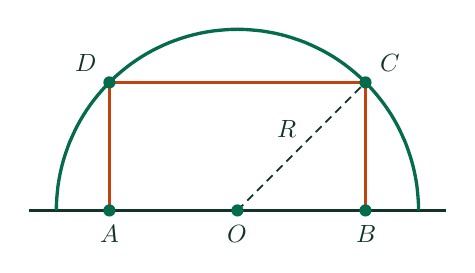
\begin{tikzpicture}
\draw[ink, line width=0.8pt] (-2.650,0.000) -- (2.650,0.000);
\draw[color={rgb,255:red,4;green,107;blue,77}, line width=1.2pt] (2.300,0.000) -- (2.299,0.080) -- (2.294,0.160) -- (2.287,0.240) -- (2.278,0.320) -- (2.265,0.399) -- (2.250,0.478) -- (2.232,0.556) -- (2.211,0.634) -- (2.187,0.711) -- (2.161,0.787) -- (2.133,0.862) -- (2.101,0.935) -- (2.067,1.008) -- (2.031,1.080) -- (1.992,1.150) -- (1.951,1.219) -- (1.907,1.286) -- (1.861,1.352) -- (1.812,1.416) -- (1.762,1.478) -- (1.709,1.539) -- (1.654,1.598) -- (1.598,1.654) -- (1.539,1.709) -- (1.478,1.762) -- (1.416,1.812) -- (1.352,1.861) -- (1.286,1.907) -- (1.219,1.951) -- (1.150,1.992) -- (1.080,2.031) -- (1.008,2.067) -- (0.935,2.101) -- (0.862,2.133) -- (0.787,2.161) -- (0.711,2.187) -- (0.634,2.211) -- (0.556,2.232) -- (0.478,2.250) -- (0.399,2.265) -- (0.320,2.278) -- (0.240,2.287) -- (0.160,2.294) -- (0.080,2.299) -- (0.000,2.300) -- (-0.080,2.299) -- (-0.160,2.294) -- (-0.240,2.287) -- (-0.320,2.278) -- (-0.399,2.265) -- (-0.478,2.250) -- (-0.556,2.232) -- (-0.634,2.211) -- (-0.711,2.187) -- (-0.787,2.161) -- (-0.862,2.133) -- (-0.935,2.101) -- (-1.008,2.067) -- (-1.080,2.031) -- (-1.150,1.992) -- (-1.219,1.951) -- (-1.286,1.907) -- (-1.352,1.861) -- (-1.416,1.812) -- (-1.478,1.762) -- (-1.539,1.709) -- (-1.598,1.654) -- (-1.654,1.598) -- (-1.709,1.539) -- (-1.762,1.478) -- (-1.812,1.416) -- (-1.861,1.352) -- (-1.907,1.286) -- (-1.951,1.219) -- (-1.992,1.150) -- (-2.031,1.080) -- (-2.067,1.008) -- (-2.101,0.935) -- (-2.133,0.862) -- (-2.161,0.787) -- (-2.187,0.711) -- (-2.211,0.634) -- (-2.232,0.556) -- (-2.250,0.478) -- (-2.265,0.399) -- (-2.278,0.320) -- (-2.287,0.240) -- (-2.294,0.160) -- (-2.299,0.080) -- (-2.300,0.000);
\draw[color={rgb,255:red,194;green,65;blue,12}, line width=1.1pt] (-1.626,0.000) -- (-1.626,1.626) -- (1.626,1.626) -- (1.626,0.000);
\draw[ink, line width=0.6pt, dash pattern=on 3pt off 2pt] (0.000,0.000) -- (1.626,1.626);
\fill[color={rgb,255:red,4;green,107;blue,77}] (-1.626,0.000) circle (2.2pt);
\fill[color={rgb,255:red,4;green,107;blue,77}] (1.626,0.000) circle (2.2pt);
\fill[color={rgb,255:red,4;green,107;blue,77}] (1.626,1.626) circle (2.2pt);
\fill[color={rgb,255:red,4;green,107;blue,77}] (-1.626,1.626) circle (2.2pt);
\fill[color={rgb,255:red,4;green,107;blue,77}] (0.000,0.000) circle (2.2pt);
\node[font=\small, text=ink, inner sep=0.5pt] at (-1.626,-0.300) {$A$};
\node[font=\small, text=ink, inner sep=0.5pt] at (1.626,-0.300) {$B$};
\node[font=\small, text=ink, inner sep=0.5pt] at (1.926,1.876) {$C$};
\node[font=\small, text=ink, inner sep=0.5pt] at (-1.926,1.876) {$D$};
\node[font=\small, text=ink, inner sep=0.5pt] at (0.000,-0.300) {$O$};
\node[font=\small, text=ink, inner sep=0.5pt] at (0.633,1.033) {$R$};
\end{tikzpicture}
\end{document}
